%%
%% This is file `mcmthesis-demo.tex',
%% generated with the docstrip utility.
%%
%% The original source files were:
%%
%% mcmthesis.dtx  (with options: `demo')
%%
%% -----------------------------------
%%
%% This is a generated file.
%%
%% Copyright (C)
%%       2010 -- 2015 by Zhaoli Wang
%%       2014 -- 2019 by Liam Huang
%%       2019 -- present by latexstudio.net
%%
%% This work may be distributed and/or modified under the
%% conditions of the LaTeX Project Public License, either version 1.3
%% of this license or (at your option) any later version.
%% The latest version of this license is in
%%   http://www.latex-project.org/lppl.txt
%% and version 1.3 or later is part of all distributions of LaTeX
%% version 2005/12/01 or later.
%%
%% This work has the LPPL maintenance status `maintained'.
%%
%% The Current Maintainer of this work is Liam Huang.
%%
%%
%% This is file `mcmthesis-demo.tex',
%% generated with the docstrip utility.
%%
%% The original source files were:
%%
%% mcmthesis.dtx  (with options: `demo')
%%
%% -----------------------------------
%%
%% This is a generated file.
%%
%% Copyright (C)
%%       2010 -- 2015 by Zhaoli Wang
%%       2014 -- 2019 by Liam Huang
%%       2019 -- present by latexstudio.net
%%
%% This work may be distributed and/or modified under the
%% conditions of the LaTeX Project Public License, either version 1.3
%% of this license or (at your option) any later version.
%% The latest version of this license is in
%%   http://www.latex-project.org/lppl.txt
%% and version 1.3 or later is part of all distributions of LaTeX
%% version 2005/12/01 or later.
%%
%% This work has the LPPL maintenance status `maintained'.
%%
%% The Current Maintainer of this work is Liam Huang.
%%
\documentclass{mcmthesis}
\mcmsetup{CTeX = false,   % 使用 CTeX 套装时,设置为 true
        tcn = 2007379, problem = E,
        sheet = true, titleinsheet = false, keywordsinsheet = true,
        titlepage = true, abstract = true}
\usepackage{newtxtext}%\usepackage{palatino}
\usepackage{lipsum}

\title{The Known Name}
\author{Team 2007379}
\date{\today}
\begin{document}
\begin{abstract}

Plastic waste (PW) has been one of intractable environmental dilemma for modern humankind. Traditionally, theories of plastic treatment focus on the amount and production of plastics with assessment of their managed impact on environment dependently. In order to migrate this tough problem, we combine producing of plastics and managing of plastic waste to establish a model to evaluate and reduce the plastic waste, then try to find out better solutions to prevent our cities from being flooded by plastic waste.

Firstly, we develop a plastic waste estimate model (PWEM) based on life cycle assessment (LCA) with consideration of certain factors ranging from the sources to the final management of PW, to estimating the maximal levels of single-use or disposable plastic products in a certain region or country. Linear programming and optimization methed are the core mathematical methods of PWEM, including one particular objective function and four  constraint conditions. We set the amount of plastics as the target value, while we dependently explore the four possible ends of PW and formulate their impacts on environment by several functions. As a result, PWVM can put out the maximal amount of plastic products by analyzing the input digits of any region. 

Secondly, to find out to what extent plastic waste can be minimized, we established an model called HSVR which combines happiness-index analysis and SVR method.  

Thirdly, we  promote our basic model to suit the international environment which can conclude an achievable minimal target level of global PW. We follow the precious happiness index to assess how much human life is changed, and apply the Environmental Assessment of Solid Waste Systems and Technologies (EASEWASTE) model to evaluating how the the environment is affected by plastic reduction. Moreover, for valuing the loss of multiple plastic industry, we take computable general equilibrium (CGE) model to quantify the negative effects of the target plastic production. Then we normalized the outputs and into indexs, and calculate the weight for each indicator above by the analytic hierarchy process (AHP). After that, we take a linear combination of variables that have been quantified to conclude the total impact for achieving the confined level. 

Furthermore, whether the plastic waste is overloaded or the plastic products are reduced, they may impact countries unequally because of their different development level.  We discuss several measures that could be taken:

\begin{enumerate}
	\item Diversifying the standard level of plastic waste based on countries’ level of development.
	\item Drawing up a plan to encourage technical support from developed to developing countries.
\end{enumerate}

Finally,  we revise our original model by add a time-dependent index -
Or: we expand a time sequence model (TSM)  -
to analyze how to approach the target minimum level following the time line by an achievable way. It should be noticed that many unexpected circumstance would definitely appear so we empirically choose most significant possibilities that may delay or accelerate the achievement process. The result are specified into a memo which can be provided for ICM.
Sensitivity analysis model testing by case analyzing.

\begin{keywords}
plastic waste; estimate; LCA model; HSVR model; EASEWASTE model; AHP
\end{keywords}
\end{abstract}
\maketitle
%% Generate the Table of Contents, if it's needed.
%% \tableofcontents
%% \newpage
%%
%% Generate the Memorandum, if it's needed.
%% \memoto{\LaTeX{}studio}
%% \memofrom{Liam Huang}
%% \memosubject{Happy \TeX{}ing!}
%% \memodate{\today}
%% \logo{\LARGE I'm pretending to be a LOGO!}
%% \begin{memo}[Memorandum]
%%   \lipsum[1-3]
%% \end{memo}
%%
\section{Introduction}
\subsection{Background}

The plastic industry can date back to1950s, over the past 60 years, the production of plastic has grown rapidly, which has surpass most other artificial materials\cite{Geyer}. While people then did not realize the potential negative influence of plastic usage to ecosystem, plastic waste gradually accumulated in the environment because of it’s non-biodegradable trait. Some scholar believe that plastic bags and Styrofoam containers can take up to 1,000 years to decompose\cite{Giacovelli}. 6,300Mt plastic waste has been generated in 2015, while only 9\% of which had been recycled and reused. 12\% of them were incinerated and the percentage of plastics that discarded in landfills or natural environment was up to 79\%\cite{Geyer}. Plastics in nature especially in the ocean will cause a series of ecological problems. Apart form the chemical affects to organisms, plastic ingestion and entanglement are also threatening the diversity of species\cite{LI}. It is easy to imagine that if no measure is taken, human will facing severe degradation and pollution caused by enormous plastic waste.

Besides, the management of the plastic waste is one of the hardest issue on integrated municipal solid waste (MSW). There are many researches that focus on the plastic recovery routes based on the life cycle assessment approach (LCA) \cite{Rigamonti}, and a few methods to assess the impact of solid waste system and technologies, which aim at develop more effective ways to migrate the plastic waste problem\cite{Kirkeby}.

However, it seems that there are few researchers ever explore the valuation model of estimating the maximum use of plastics nor utility policy to reduce the usage of plastics remarkably. That indicates there is still room for further explanation in this area. 

The management of the plastic waste is one of the most controversial topic in the discussion on integrated municipal solid waste area.

\subsection{Restatement of the problem}

Living in the age that are characterized by a series of  troublesome environmental problems, such as global warming, desertification, pollution of water and poor air quality. Our team is hired to estimate the maximal permitted amount of plastic products, migrate the plastic production and reduce plastic waste. In another word, we need to answer the following questions:

\begin{enumerate}
	\item What is the maximal level of single-use or disposable plastic products without further pollution?
	\item What extent can plastic waste be reduced to?
	\item What is the minimal achievable level of global single-use or disposable plastic products and what are the impact on certain facets of reaching this level?
	\item How to solve the equity problem about plastic waste that arise from global crisis?
	\item How to build a timeline to approuch our target level we set before and describe our exploration to ICM?
\end{enumerate}

\subsection{Overview of our work}

For task 1, we build PWEM on the basis of LCA, and applied some logical abstractions, physical derivations, and mathematical methods to accomplished the linear programming process, then out put the estimated maximal level of plastic products. 

For task 2,  considering the shortage of data, we create our HSVR model to define the miximal level with least negative effects on people’s  living standards. 

For task 3, we set an achievable target level of plastic usage and apply quite a few known methods to quantify and combine the given factors for assessing the total influence of achieving our goal. 

For task 4, we revise our model and provide realistic solutions for the mentioned euity issue.

For task 5, TSM is established for predicting the possible timeline and discuss possible relevant circumstances, then write a specific memo for ICM.

\section{Assumptions and justifications}

To simplify the problem, we strive for the following assumptions:

\begin{itemize}
	
	\item \textbf{The mass of annual plastic production equals to that of the annual plastic waste.} On the one hand, every pounds of plastic produced will turn into waste. On the other hand, the lifeline of most sorts of plastic is under 20 so that given situation will not change acutely\cite{Geyer}.
	
	\item \textbf{Throughout the life cycle of plastic, the impact of plastic on environment in use phase is negligible.} Main environment issues are related to plastic merely when it is produced or managed\cite{book}.
	
	\item \textbf{Aiming to make plastic waste safely be mitigated, any waste should be landfilled.} It’s extremely hard for plastic to break down in landfills. And the current circumstance is that, in many countries, America for example, available landfill capacity is about to run out\cite{book}.
	
	\item \textbf{All the plastic waste produced will be managed.} In the long run, the NET plastic waste discarded in natural environment will approach zero by governments and NGOs’ efforts.
	
	\item \textbf{The proper quantity of pollutant emission of plastic waste should depend on the contribution of plastic industry to the gross domestic products.} In fact, the pollutant emission of plastic waste is just a ordinary part of the total emission, so the responsibility of environmental protection it takes should also be the proportional part, which is roughly estimated by the percentage of GDP plastic industry contributes.
	
\end{itemize}

\section{A model for maximal plastic waste estimation}

\subsection{LCA analysis}

Plastic waste impacts the environment in different life phases(particularly production and management). Therefore the environmental impact assessment has been carried out using life cycle assessment (LCA) approach so that we can estimate the maximum levels of single-use or disposable plastic product waste.

\subsection{Qualify the impact on the environment}

According to the first assumption, we consider the annual production and waste as the same variable $S$. And naturally it is divided into various sorts of plastic.

\begin{equation}
S = \sum_i{s_i}
\label{S}
\end{equation}

Note that, $i$ represents a sort of plastic and  $s_i$ is the annual production of this sort of plastic.

To quantify to what extent plastic waste impact the environment in its life cycle, we use Units of polluted water ($UPW$) and air ($UPA$) to measure emissions. UPW is the number of cubic meters of water polluted up to the European drinking water standard by the production of 1 tonne of the material. UPA is a similar measure for air and gives the cubic meters of air needed to dilute the emissions to the European maximum acceptable concentration (MAC)\cite{book}. Then the Emissions of water($EW$) and air ($EA$) can be formulated below:

\begin{equation}
EA^{\alpha} = \sum_i{s_i}\times UPA_i^\alpha
\label{EA}
\end{equation}

\begin{equation}
EW^{\alpha} = \sum_i{s_i}\times UPW_i^\alpha
\label{EW}
\end{equation}

Note that the superscript $\alpha$ means the process of plastic production. Similarly, replace $\alpha$ with $\beta$ means the process of plastic waste management.

When it comes to plastic waste management, there are three possible fates for managed plastic waste: be recycled, be incinerated or be discarded(be landfilled or be discarded in natural environment). According to the third and fourth assumption, we don’t take the part of waste discarded into account. And the proportion of the recycled part and the incinerated part(symbolized by ) is given by scenario P4 in paper\cite{Rigamonti}. Then the environmental impact of plastic waste management can be calculated:

\begin{equation}
EA^\beta = \frac{\sigma}{1+\sigma}\sum_i{s_i}\times UPA_i^\beta
\label{EAB}
\end{equation}

\begin{equation}
EW^\beta = \frac{\sigma}{1+\sigma}\sum_i{s_i}\times UPW_i^\beta
\label{EWB}
\end{equation}

Additionally, in the process of incineration, we take the Emission of greenhouse gases CO2($EC$) into account.

\begin{equation}
EC = \frac{\sigma}{1+\sigma}\sum_i{s_i}\times N_i
\label{EC}
\end{equation}

where $N_i$ is the number of $CO_2$ generated by the combustion of 1 molecule specific plastic unit. The superscript $\beta$ is omitted because only the incineration process emit $CO_2$.

Apart from above analysis, although we assume that all the plastic waste discarded in natural environment will be managed, too much plastic waste discarded(even if temporarily) will notably do harm to marine ecosystem\cite{LI}. Thus it’s necessary to estimate the mass of plastic waste(symbolized by $SM$) inputs from land into the ocean, given specific total plastic waste.

\begin{equation}
SM = \varsigma\sum_i{s_i}
\label{SM}
\end{equation}

$\varsigma$ is the empirical coefficient of $SM$ and total mass of plastic waste, calculated by former statistics.

\subsection{Constraints given by environmental carrying capacity}

Firstly, according to the fifth assumption, the pollutant emission constraints are roughly estimated by the percentage of GDP plastic industry contributes, quantified by coefficient $\theta$.

\begin{equation}
EA^\alpha + EA^\beta \le \theta V_{air}
\label{air}
\end{equation}

\begin{equation}
EW^\alpha + EW^\beta \le \theta V_{water}
\label{water}
\end{equation}

$V_{air}$ and $V_{water}$ is the total available air/water of a specific country/region.

Secondly, when it comes to greenhouse gas $CO_2$, it’s more propriate to use its fossil fuel consumption percentage to set the restraint because the fossil fuel combustion is the principal factor of the global warming, rather than natural carbon cycles\cite{book}.

\begin{equation}
EC \le \iota V_{CO_2}
\label{ECO}
\end{equation}

where $V_{CO_2}$ is the promised maximal $CO_2$ emissions of specific country or region and $\iota$ is fossil fuel consumption percentage. Generally, $\iota$ equals 4\%.

Last but not least, considering current quantity of plastic discarded in the ocean don’t exert severe impact on marine ecosystem, we regard zero net input into the sea an acceptable circumstance for marine environment, i.e. annual plastic waste input can’t beyond the quantity of annual management of marine plastic(symbolized by $M$).

\begin{equation}
SM \le M
\end{equation}

Finally, we can synthesize the formulas above, solve the constrained optimization problem and obtain the maximum levels of plastic product waste.

\section{To what extent plastic waste can be reduced}

\label{p2}

At present, the global use of plastics has exceeded the upper limit of environmental tolerance, which poses a huge threat to the ecological environment. In section \ref{p2}, We propose a model of Happiness based on SVR\cite{Smola}, which we call HSVR. Using HHSVR, we will explore the impact of the use of plastic on human living standards, and try to reduce the amount of plastic used as much as possible without affecting much of human living standards.

Our starting point is straightforward: the use of plastic is essential, and reducing the use of plastic will inevitably affect the living standards of local people. By analyzing the characteristics of different regions (especially the amount of plastics produced) and the people's living standards, we find out the relationship between the amount of plastics produced and the people's happiness index. Based on this, we can analyze how much plastic production we can reduce without significantly reducing the happiness index.

The following of this section will first briefly introduce the method we use, and then obtain a specific regression model based on the Global Happiness Report\cite{World} and plastic production in each region\cite{Plastic}.

\subsection{SVR algorithm}

Support vector regression(SVR) is an application of SVM (support vector machine) to regression problems. Support vector machines construct a hyperplane or a series of hyperplanes in a high-dimensional or infinite-dimensional space, which can be used for classification, regression, or other tasks. Intuitively, using a hyperplane to achieve a good segmentation can make the closest training data points have the largest separation distance in any category. This is because usually a larger margin can have a lower generalization error of classifier\cite{SVRs}.

Given training vectors $x_i \in R^p, i = 1, \cdots, n$, and a vector $y \in R^n$. $\varepsilon-SVR$ solves the following primal problem:

\begin{equation}
\min_{\omega,b,\zeta,\zeta^*}\frac{1}{2}\omega^T\omega + C \sum_{i = 1}^n(\zeta_i + \zeta_i^*) 
\label{primal}
\end{equation}

subject to 

\begin{equation}
y_i - \omega^T\phi(x_i) - b \le\varepsilon + \zeta_i
\label{sub1}
\end{equation}

\begin{equation}
\omega^T\phi(x_i) + b - y_i \le\varepsilon + \zeta_i^*
\label{sub2}
\end{equation}

where $\zeta_i, \zeta_i^* \ge 0, i = 1, \cdots, n$.

Its dual is

\begin{equation}
\min_{\alpha,\alpha^*}\frac{1}{2}(\alpha-\alpha^*) + \varepsilon e^T(\alpha + \alpha^*) - y^T(\alpha-\alpha^*)
\label{dual}
\end{equation}

subject to 

\begin{equation}
e^T(\alpha - \alpha^*) = 0
\label{sub4}
\end{equation}

where $0 \le \alpha_i, \alpha_i^* \le C, i = 1, \cdots, n$, $e$ is the vector of all ones, $C > 0$ is the upper bound, $Q$ is an $n$ by $n$ positive semidefinite matrix, $Q_{ij} \equiv K(x_i, x_j) = {\phi(x_i)}^T\phi(x_j)$ is the kernel. Here training vectors are implicitly mapped into a higher (maybe infinite) dimensional space by the function $\phi$. $\phi$ can be linear, polynomial, sigmoid or others.

The decision function is:

\begin{equation}
\sum_{i = 1}^{n}(\alpha_i - \alpha_i^*)K(x_i,x) + \rho
\label{decision}
\end{equation}

For more details, please refer to \cite{Smola}.

\subsection{Detailed analysis}

In this section, we will introduce the quantitative standard of happiness, analyze this problem, and use SVR to get the function of happiness and plastic production $\hat{f}$ so that $\hat{f}: X \mapsto y$, where $X$ is a vector in $\mathcal{X} = \mathcal{R}^d$, including a dimension of plastic production.

\subsubsection{The quantitative standard of happiness}

We use the happiness quantification standard used by the World Happiness Report\cite{World}, where the happiness scores and rankings use data from the Gallup World Poll. The scores are based on answers to the main life evaluation question asked in the poll. This question, known as the Cantril ladder, asks respondents to think of a ladder with the best possible life for them being a 10 and the worst possible life being a 0 and to rate their own current lives on that scale. The scores are from nationally representative samples for the years 2013-2016 and use the Gallup weights to make the estimates representative. 

Obviously, people's happiness depends not only on the amount of plastic produced. In fact, plastic production and waste account for only a small part of the factors affecting people's happiness. There are six factors usually concerned to be relevant to happiness: economic production, social support, life expectancy, freedom, absence of corruption, and generosity. The data that estimates the extent to which each of six factors contribute to making life evaluations higher in each country than they are in Dystopia, a hypothetical country that has values equal to the world’s lowest national averages for each of the six factors, is also used to as part of the input of HSVR, with some preprocessing:

\begin{equation}
x^* = \frac{x - x_{min}}{x_{max} - x_{min}}
\label{toone}
\end{equation}

where $x_max,x_min$ is the maximum and minimum of the original data, respectively.

Note that the first preprocessing maps the data to $[0,1]$. The preprocessing step will erase the differences between the data formats and make the characteristics of the data more obvious.

\subsubsection{Plastic Emphasized}

The impact of the production and use of plastic on happiness should be far less than that of the other six factors mentioned above, which means that the input to the problem should be a weighting of all seven factors:

\begin{equation}
X = (\epsilon_1 x_1, \epsilon_2 x_2, \epsilon_3 x_3, \epsilon_4 x_4, \epsilon_5 x_5, \epsilon_6 x_6, \epsilon_7 x_7)
\end{equation}

However, what we need to find is mainly the relationship between plastic production and happiness, so we give plastic production a sufficiently high weight, where $\epsilon_i = 1, i = 1, \cdots, n$.

The lack of data\cite{lack} in research on plastic production and consumption has always been a serious problem. To the best of our knowledge, there are no specific statistics on the amount of plastic used in many regions, especially in developing countries. This means that our research will face problems of insufficient data volume and potential data imbalances. Based on this, we chose SVR as our classifier, because SVR has the following characteristics\cite{SVRs} and is suitable for solving this problem:

\begin{itemize}
	\item Effective in high dimensional spaces.
	\item Still effective in cases where number of dimensions is greater than the number of samples.
	\item Versatile: different Kernel functions can be specified for the decision function.
\end{itemize}

\subsection{Model parameter selection}
\label{train}
We randomly selected 20 countries from \cite{World} and \cite{Plastic} as our training set as our training set. These countries include countries that consume more plastic, such as China and India, and developed countries, such as the United States and the United Kingdom. In combination with the training situation, we adjusted the model in real time to obtain the optimal model.

\subsubsection{Model performance evaluation}

To evaluate the performance of the model, we used k-fold cross-validation\cite{kf}. In k-fold cross-validation, the original sample is randomly partitioned into k equal sized subsamples. Of the k subsamples, a single subsample is retained as the validation data for testing the model, and the remaining k − 1 subsamples are used as training data. The cross-validation process is then repeated k times, with each of the k subsamples used exactly once as the validation data. The k results can then be averaged to produce a single estimation. The advantage of this method is that all observations are used for both training and validation, and each observation is used for validation exactly once. 10-fold cross-validation is commonly used\cite{McLachlan}, but in general k remains an unfixed parameter.

We choose the Euclidean norm of the regression value and the true value(or the mean square error, $MSE$) to measure the quality of the regression result:

\begin{equation}
MSE = \frac{1}{k}{\|y-\hat{y}\|}_2
\end{equation}

where $y$ is the true value, and $\hat{y}$ is the regression value.

\subsection{Specific model parameters}

We have implemented four kinds of kernel function\cite{SVRs} of SVR and verified them separately. 

The four cores are:

\begin{itemize}
	\item linear: $\langle x,x^\prime \rangle$
	\item polynomial: ${(y\langle x,x^\prime \rangle + r)}^d$.
	\item rbf: $e^{-\gamma{\|x-x^\prime\|}^2}$.
	\item sigmoid: $\tanh(\langle x,x^\prime \rangle + r)$.
\end{itemize}

Due to the high feature dimension of our training set and the small number of training samples, in general, the effect of the linear kernel should be better. The results in figure \ref{fig1} also illustrate this:

\begin{figure}[!htb] %H为当前位置,!htb为忽略美学标准,htbp为浮动图形
	\centering %图片居中
	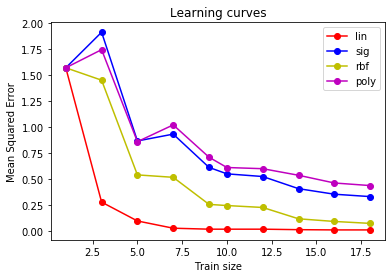
\includegraphics[width=0.7\textwidth]{figures/learncurve.png} %插入图片,[]中设置图片大小,{}中是图片文件名
	\caption{Training results of different SVR kernel functions.} %最终文档中希望显示的图片标题
	\label{fig1} %用于文内引用的标签
	
\end{figure}

As can be seen from the figure, the results of linear and rbf are much better than the results of sigmoid and polynomial, which all converge to an error close to 0. In fact, the training error of the linear kernel is on the order of $10^{-2}$. Moreover, the linear kernel has already converged by training about ten samples, which shows that our data volume is sufficient for our model.

\subsection{Predict minimum plastic usage in an area}

From the above analysis, we find that the linear kernel function has the best fitting effect, indicating that the plastic consumption has a linear relationship with the living standard. This is consistent with per capita plastic consumption in different regions. Table \ref{consumption} is a table of plastic consumption in different regions. Intuitively, the consumption of plastic is positively related to the living standard of the region. Developed regions generally have higher plastic consumption. Of course, this is also related to other factors. These are reflected in our model.

\begin{table}[]
	\center
	
	\caption{Plastic consumption in different regions}
	\begin{tabular}{|c|c|}
		\hline
		\textbf{Area}              & \textbf{\begin{tabular}[c]{@{}c@{}}Plastic consumption\\ (1 ton per 100,000 people)\end{tabular}} \\ \hline
		China                      & 1316.1                                                                                            \\ \hline
		North America              & 1571.9                                                                                            \\ \hline
		Asia Pacific               & 657.1                                                                                             \\ \hline
		Western Europe             & 2870.6                                                                                            \\ \hline
		India                      & 251.9                                                                                             \\ \hline
		Middle East                & 580.4                                                                                             \\ \hline
		Central and South America  & 308.8                                                                                             \\ \hline
		Central and Eastern Europe & 1468.4                                                                                            \\ \hline
		Africa                     & 99.8                                                                                              \\ \hline
		Japan                      & 812.9                                                                                             
		\label{consumption}
		\\ \hline
	\end{tabular}
\end{table}

Based on this conclusion, we found that reducing the amount of plastic used will inevitably affect people's happiness. Therefore, we need to make a compromise between happiness and environment. This is undoubtedly a very painful thing. Therefore, we need to find a threshold on the tolerance of the regions $\kappa$. $\kappa$ is such a value: in a specific area, if happiness $\Gamma = \hat{f}(X) < \kappa$, it is not worthwhile to reduce consumption. Note that $\hat{f}$ is trained in section \ref{train}. $\kappa$ can be derived from historical data and is closely related to each place.

Unfortunately, many people are unwilling to pay a lot for environmental protection\cite{unf}, as is shown in figure \ref{fig3}. So we carefully set this value to 1\% of the existing happiness index.

\begin{figure}[!htb] %H为当前位置,!htb为忽略美学标准,htbp为浮动图形
	\centering %图片居中
	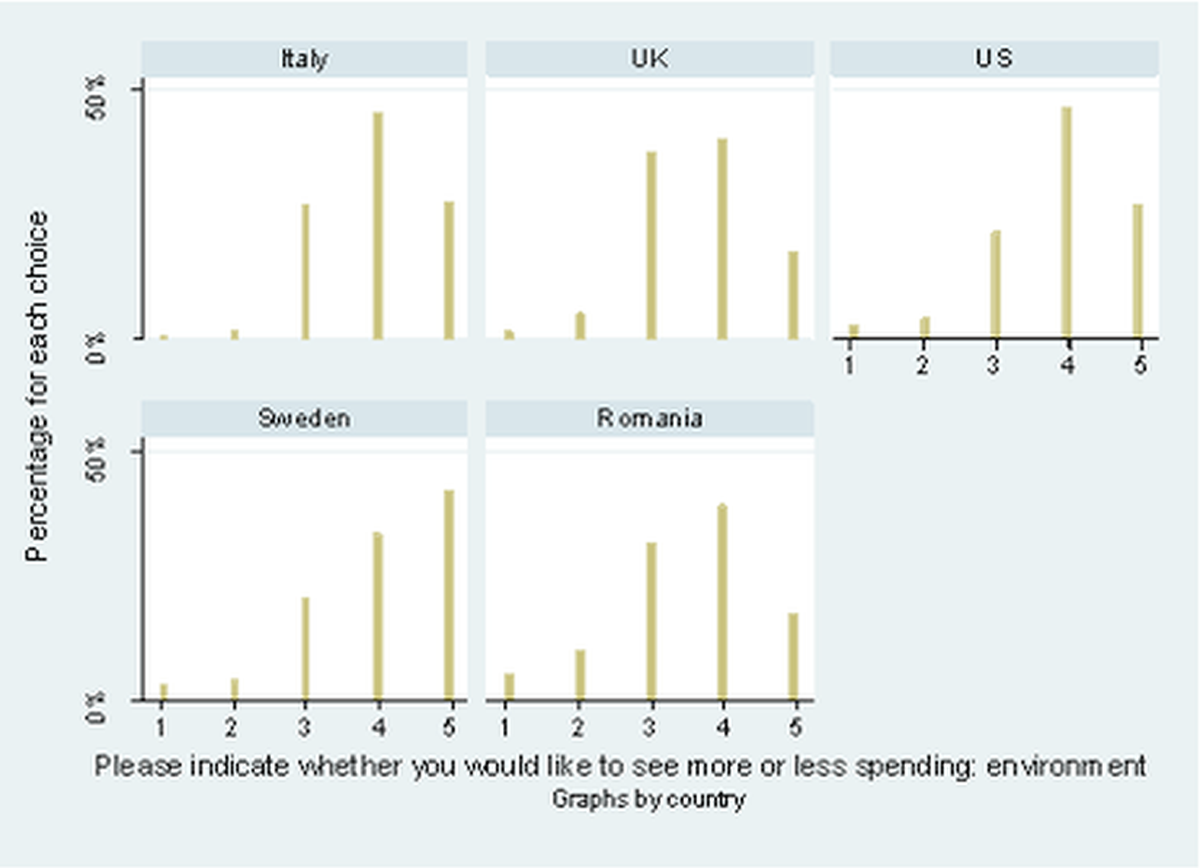
\includegraphics[width=0.7\textwidth]{figures/en.PNG} %插入图片,[]中设置图片大小,{}中是图片文件名
	\caption{Happiness-Plastic curve of US.} %最终文档中希望显示的图片标题
	\label{fig3} %用于文内引用的标签
	
\end{figure}

For example, figure \ref{fig2} shows this relationship in the US. Currently, plastic consumption in the United States is 1571.9 tons per 100,000 people. If America's tolerance for happiness is 7.263, then the minimum plastic consumption in the United States should be 500 tons per 100,000 people. If plastics production is required to fall below this limit, it will cause more problems and outweigh the benefits.

\begin{figure}[!htb] %H为当前位置,!htb为忽略美学标准,htbp为浮动图形
	\centering %图片居中
	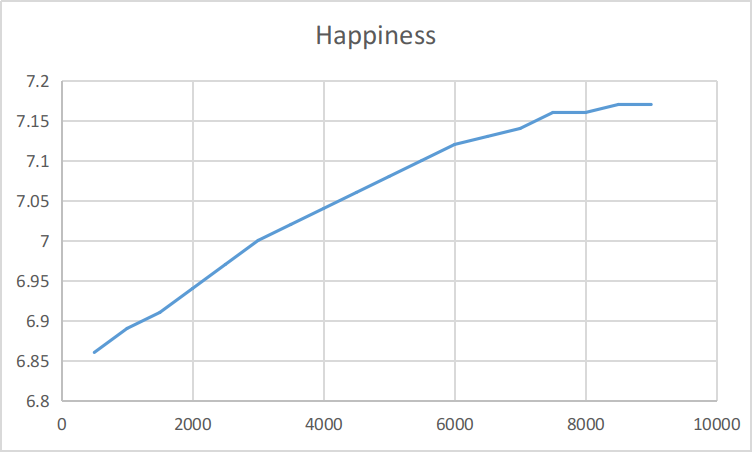
\includegraphics[width=0.7\textwidth]{figures/happiness.png} %插入图片,[]中设置图片大小,{}中是图片文件名
	\caption{Happiness-Plastic curve of US.} %最终文档中希望显示的图片标题
	\label{fig2} %用于文内引用的标签
	
\end{figure}

%We can see from figure \ref{fig2} that using too little plastic can seriously affect people's happiness. Therefore, we can set a threshold to get the smallest amount of plastic that can be used in an area.

%Our solution to this problem is based on the assumption that people will not lead a very difficult life for the reduction of plastic. Based on this, each region has its own minimum tolerable quality of life. By bringing this data into the classifier, we can get the results.

\begin{thebibliography}{99}
\bibitem{Geyer} Geyer, Roland, Jenna R. Jambeck, and Kara Lavender Law. "Production, use, and fate of all plastics ever made." Science advances 3.7 (2017): e1700782.
\bibitem{Giacovelli} Giacovelli, Claudia. "Single-Use Plastics: A Roadmap for Sustainability." (2018).
\bibitem{LI}LI, Wai Chin, H. F. Tse, and Lincoln Fok. "Plastic waste in the marine environment: A review of sources, occurrence and effects." Science of the Total Environment 566 (2016): 333-349.
\bibitem{Rigamonti}Rigamonti, Lucia, et al. "Environmental evaluation of plastic waste management scenarios." Resources, Conservation and Recycling 85 (2014): 42-53.
\bibitem{Kirkeby}Kirkeby, Janus T., et al. "Environmental assessment of solid waste systems and technologies: EASEWASTE." Waste Management \& Research 24.1 (2006): 3-15.
\bibitem{Smola}Smola, Alex J., and Bernhard Schölkopf. "A tutorial on support vector regression." Statistics and computing 14.3 (2004): 199-222.
\bibitem{World}World Happiness Report. https://kaggle.com/unsdsn/world-happiness. Accessed 15 Feb. 2020.
\bibitem{Plastic}“Plastic Industry Worldwide.” Statista, https://0-www-statista-com.lib.rivier.edu/study/51465/global-plastics-industry/. Accessed 15 Feb. 2020.
\bibitem{SVRs}1.4. Support Vector Machines — Scikit-Learn 0.22.1 Documentation. https://scikit-learn.org/stable/modules/svm.html. Accessed 15 Feb. 2020.
\bibitem{lack}Groot, Jim, et al. "A comprehensive waste collection cost model applied to post-consumer plastic packaging waste." Resources, Conservation and Recycling 85 (2014): 79-87.
\bibitem{book}Andrady, Anthony L., ed. Plastics and the Environment. John Wiley \& Sons, 2003.
\bibitem{kf}“Cross-Validation (Statistics).” Wikipedia, 7 Feb. 2020. Wikipedia, https://en.wikipedia.org/w/index.php?title=Cross-validation\_(statistics)\&oldid=939673086.
\bibitem{McLachlan}McLachlan, Geoffrey J., Kim-Anh Do, and Christophe Ambroise. Analyzing microarray gene expression data. Vol. 422. John Wiley \& Sons, 2005.
\bibitem{unf}Arpad, Todor. “Willing to Pay to Save the Planet? Evaluating Support for Increased Spending on Sustainable Development and Environmentally Friendly Policies in Five Countries.” PLOS ONE, vol. 13, no. 11, Nov. 2018, p. e0207862. PLoS Journals, doi:10.1371/journal.pone.0207862.


\end{thebibliography}


\end{document}
%%
%% This work consists of these files mcmthesis.dtx,
%%                                   figures/ and
%%                                   code/,
%% and the derived files             mcmthesis.cls,
%%                                   mcmthesis-demo.tex,
%%                                   README,
%%                                   LICENSE,
%%                                   mcmthesis.pdf and
%%                                   mcmthesis-demo.pdf.
%%
%% End of file `mcmthesis-demo.tex'.
